\chapter{Results and Discussion}

\section{Thin film characterization}
\subsection{Images from optical microscopy}

Figure \ref{fig:hpo} shows images of thin films under a $40\times$ magnification.
From the images it can be observed that material does not completely cover the whole substrate.
Moreover, the distribution of the particles was random, as was verified by image analysis techniques from the MKS framework in a later discussion.

\begin{figure}
  \centering
  \begin{subfigure}{.8\textwidth}
    \centering
    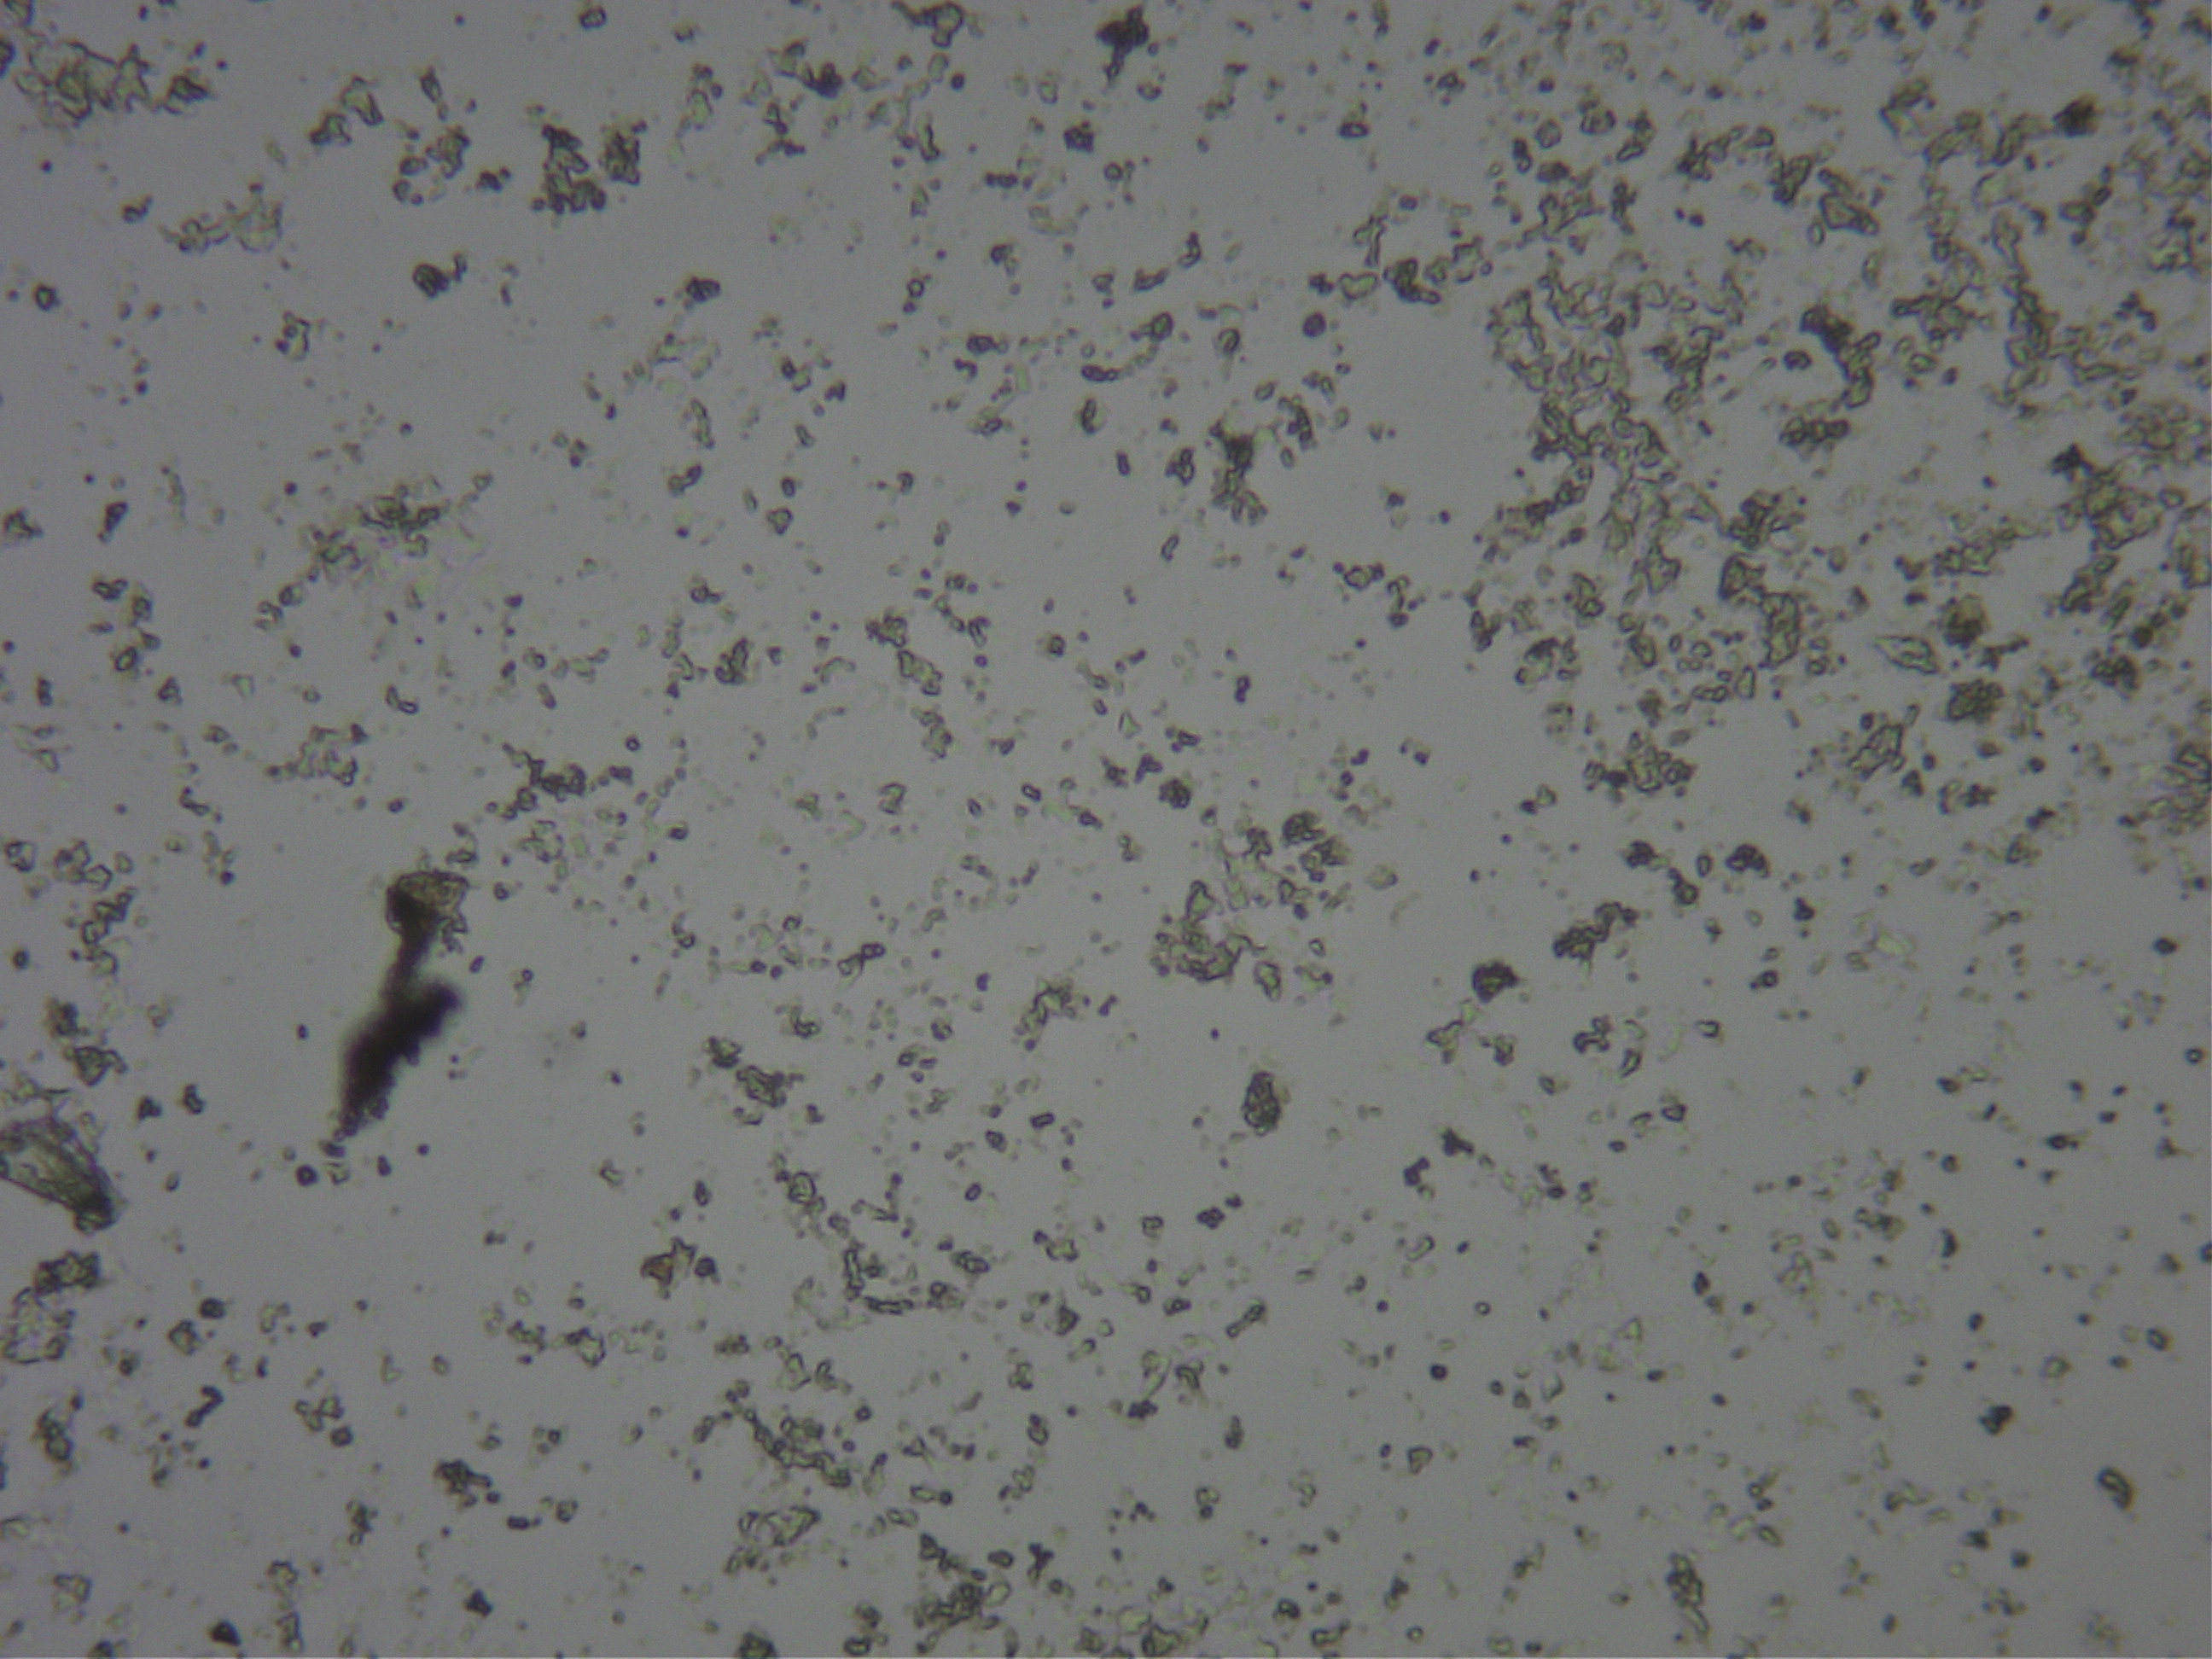
\includegraphics[scale=0.1]{s2.JPG}
    \caption[Dark areas in films]{An image capturing one material state. It can be seen that there are dark areas.}
    \label{fig:dark}
  \end{subfigure}
  \begin{subfigure}{.8\textwidth}
    \centering
    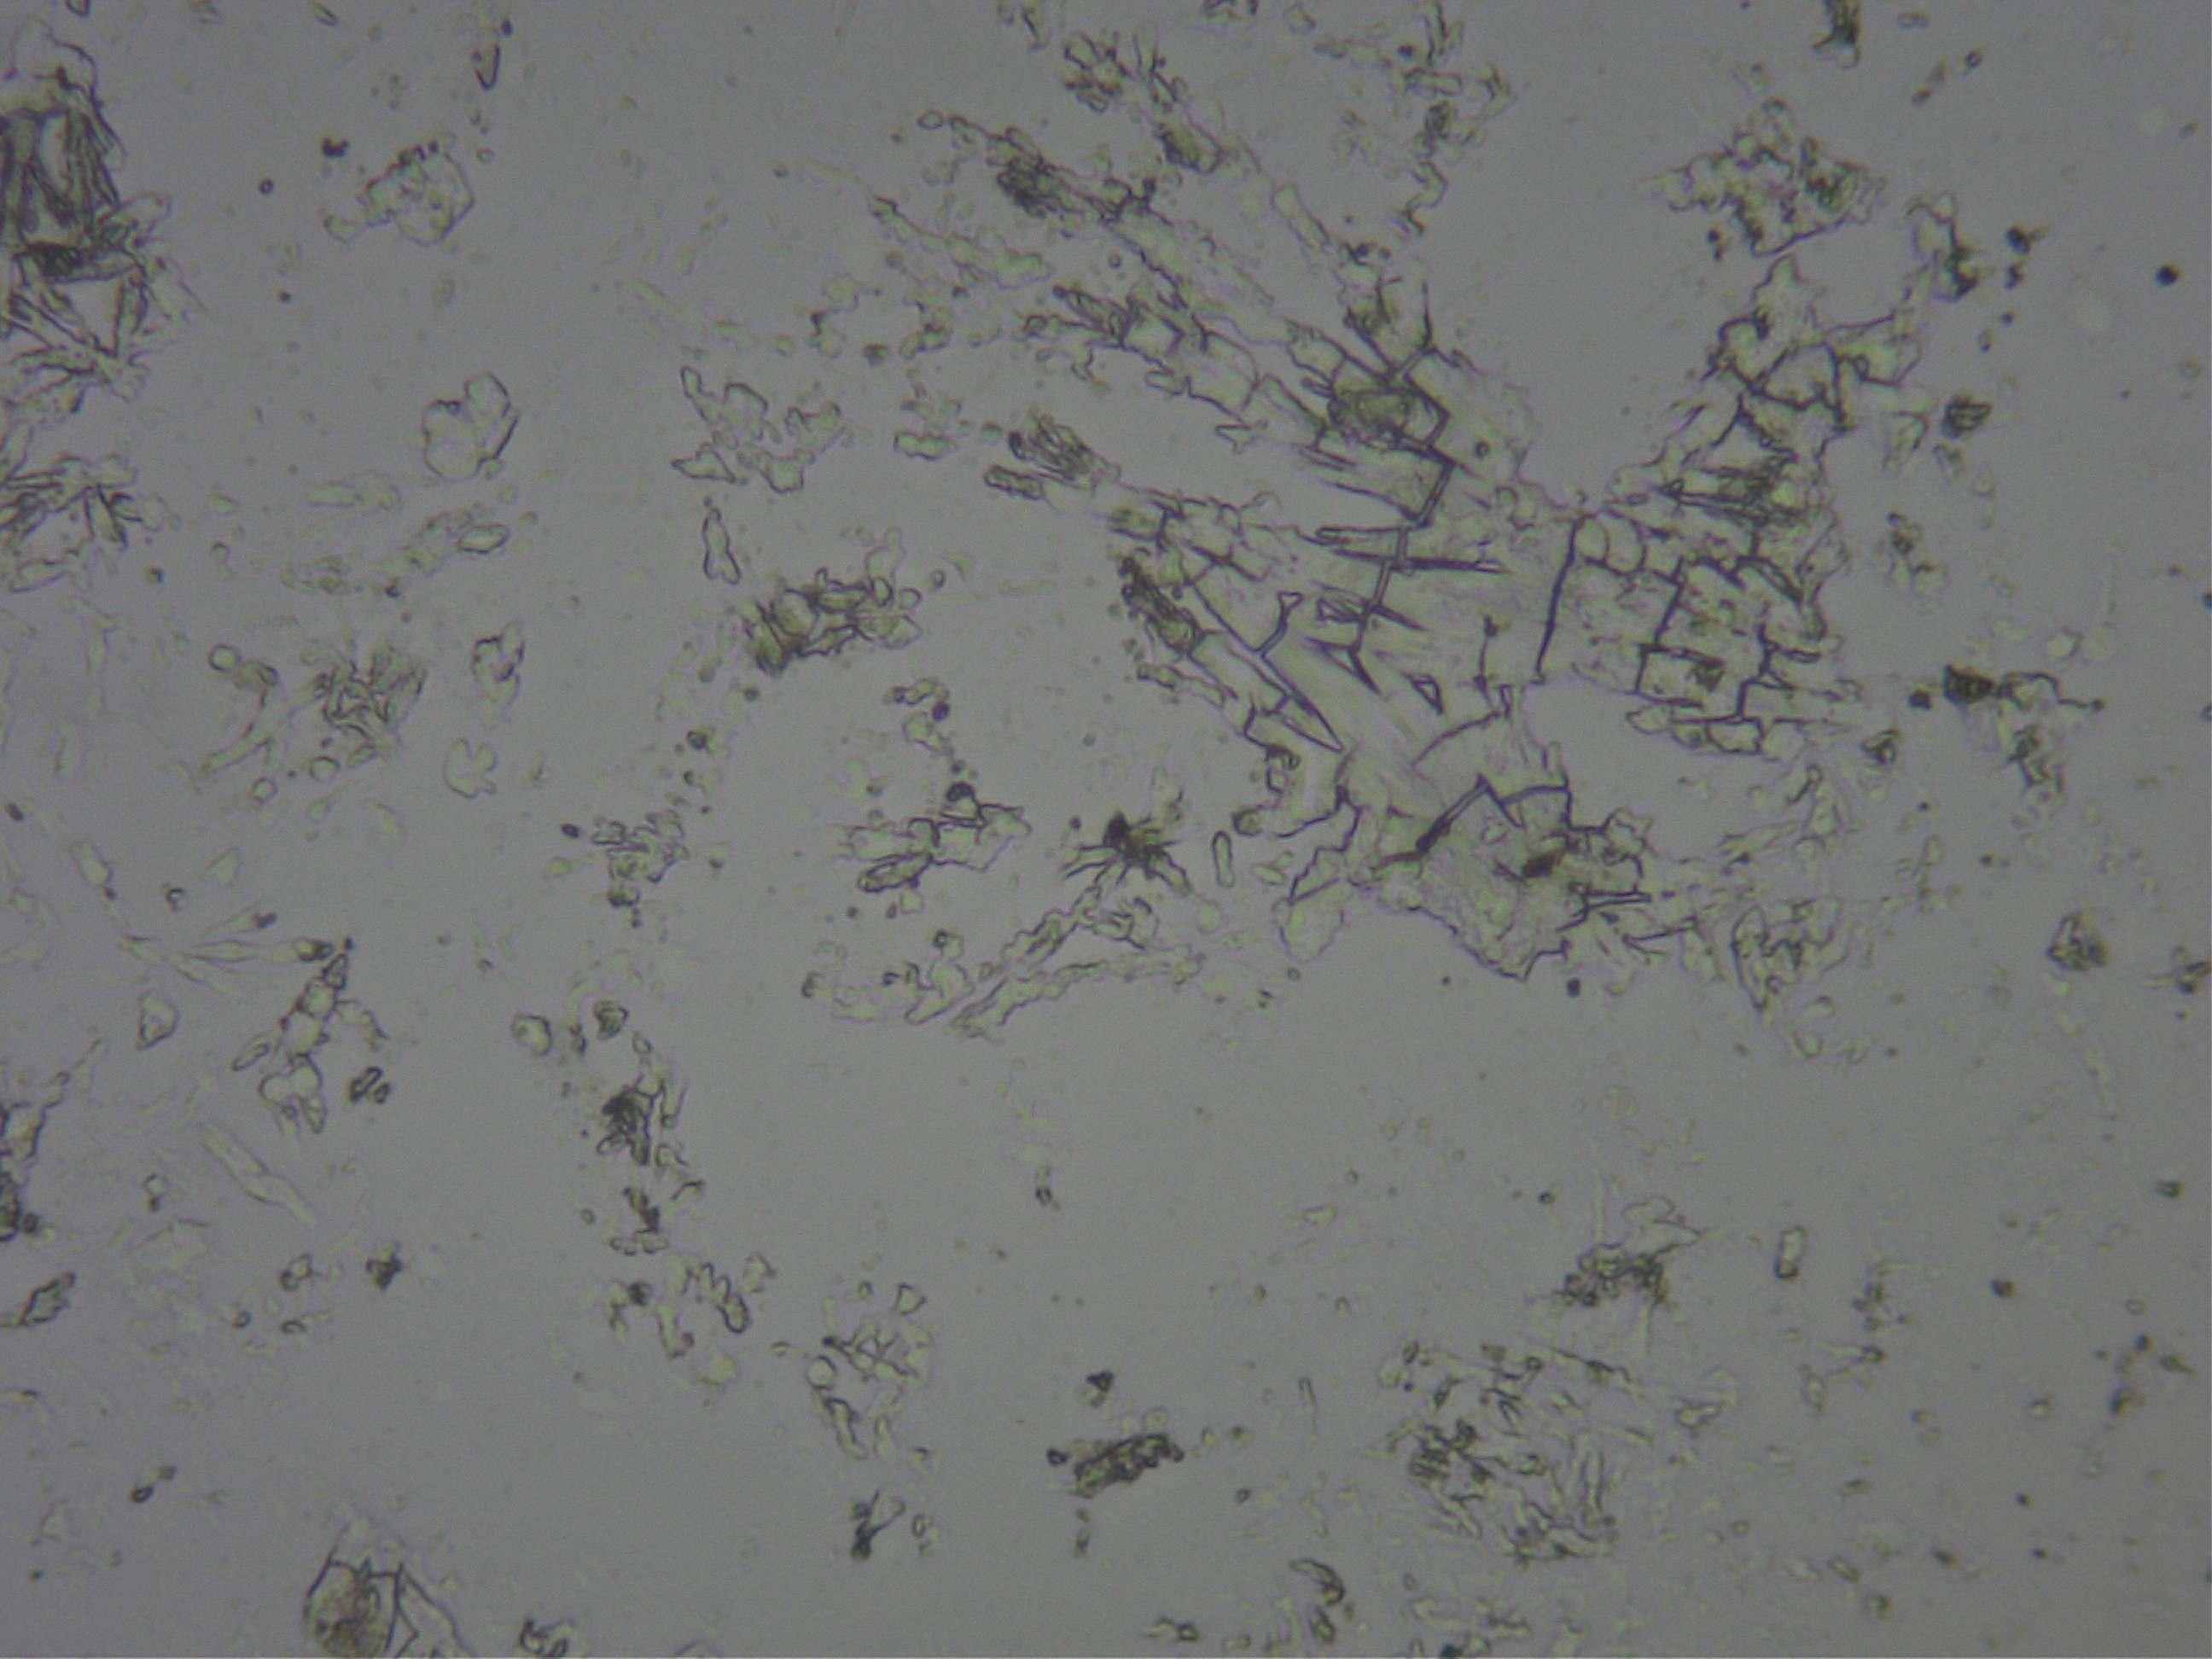
\includegraphics[scale=0.1]{s3.JPG}
    \caption[Light areas in films]{An image capturing another material state. It can be seen that there are light areas shaped like flakes.}
    \label{fig:light}
  \end{subfigure}
  \caption[HPO images of films]{Images taken using high poewr objective lens of a digital compound microscope. It can be seen that there are dark colored areas in Figure \ref{fig:dark} and light colored areas in Figure \ref{fig:light}}
  \label{fig:hpo}
\end{figure}

This means that \textbf{no} accurate measurements about the specific properties of the material can be measured in the length scale.
In order to measure the resistivity of the material, for example, it is important that the material completely covers the length from the current source and sink for four-point probe sensing.
Since there are spaces between material structures, electrical resistance is increased by the interaction with glass.
It can be said that the formation of material using the processes specified were not able to yield replicable results.

\subsection{Images from scanning electron microscopy}

Figure \ref{fig:sem} shows images of thin films under multiple magnification levels.
One of the images show the side profile of one of the thin films showing its thickness.
% check this value later on
The thickness of the film is reported to be $\SI{50}{\micro\meter}$.
% also look for the results of the other researchers on their values for thin film thickness and compare the values.
Comparing to \citeA{florido17}, the thickness of the fabricated thin film was reported to be $\SI{50}{\micro\meter}$.
This indicates that the processes used produced films of similar thickness despite the difference in number of deposition cycles used.

\begin{figure}
  \centering
  \begin{subfigure}{.5\textwidth}
    \centering
    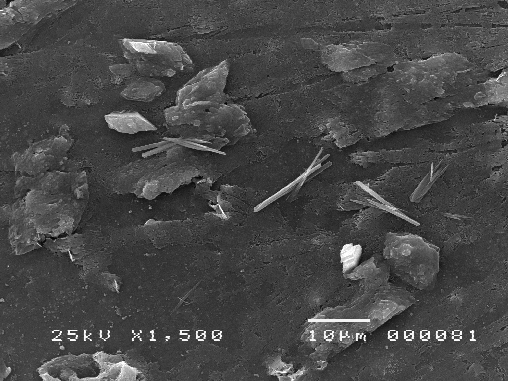
\includegraphics[scale=0.4]{dist.png}
    \caption{SEM image taken at $1500\times$ showing distribution of objects in the substrate}
    \label{fig:dist}
  \end{subfigure}
  \begin{subfigure}{.5\textwidth}
    \centering
    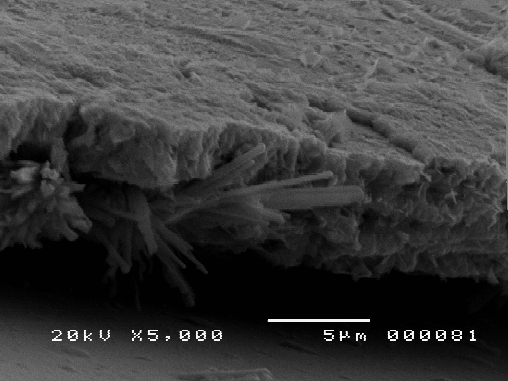
\includegraphics[scale=0.4]{thicc.png}
    \caption{SEM image taken at $5000\times$ showing thickness of film layer}
    \label{fig:thicc}
  \end{subfigure}
  \begin{subfigure}{.5\textwidth}
    \centering
    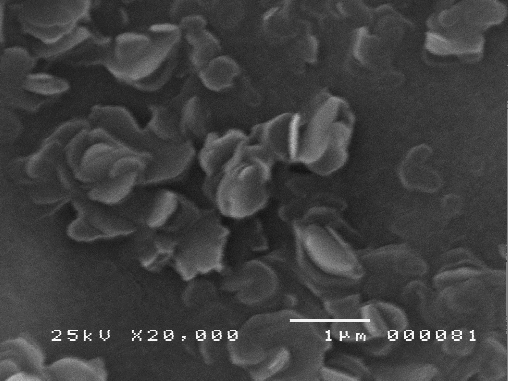
\includegraphics[scale=0.4]{flex.png}
    \caption{SEM image taken at $20000\times$ showing zinc oxide crystals}
    \label{fig:flex}
  \end{subfigure}
  \caption[Material images under SEM]{Material images taken under scanning electron microscope at different magnification values. The images show the crystals present, particle distribution, and film thickness.}
  \label{fig:sem}
\end{figure}

\subsection{Energy dispersive spectroscopy analysis}

Figure \ref{fig:edx} shows the EDX spectra showing the different atoms present in a part of the sample.

% replace figure as soon as possible
\begin{figure}
  \centering
  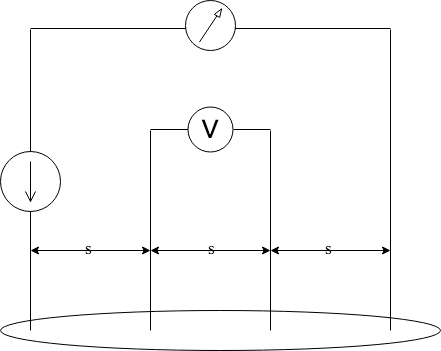
\includegraphics[scale=0.3]{FourPoint.png}
  \caption[EDX spectra of thin films]{Energy dispersive spectroscopy spectra of sections in thin film samples.}
  \label{fig:edx}
\end{figure}

\subsection{Structure elucidation from x-ray diffraction}

Figure \ref{fig:xrd} shows the x-ray diffraction spectra of the thin films.

% replace figure as soon as possible
\begin{figure}
  \centering
  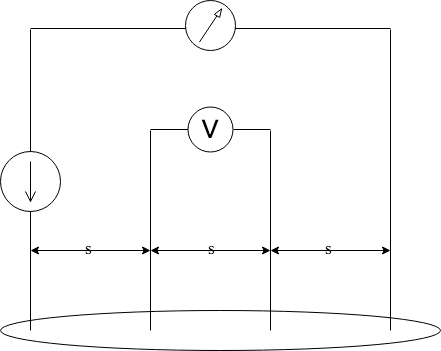
\includegraphics[scale=0.3]{FourPoint.png}
  \caption[XRD spectra of ]{X-ray diffraction spectra of thin film samples}
  \label{fig:xrd}
\end{figure}

\subsection{Four-point probe sensing}

Table \ref{tab:fps} shows the average sheet resistance values along with the statistical range.

% replace table content as soon as possible.
\begin{table}
  \centering
  \begin{tabular}{ c c c }
    \hline
    \hline
    1 & 2 & 3 \\
    4 & 5 & 6 \\
    \hline
  \end{tabular}
  \label{tab:fps}
\end{table}

\section{Development of materials knowledge framework}
\subsection{Calculation of two point spatial correlations}

Two point spatial correlations (autocorrelations) were calculated based on two main material phases as seen in the optical microscopy images: the presence and absence of zinc oxide in the structure.
Contour plots showing the statistics are shown in Figure \ref{fig:spat}.

\begin{figure}
  \centering
  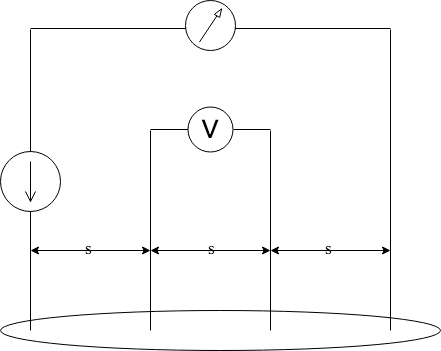
\includegraphics[scale=0.4]{FourPoint.png}
  \caption[Contour plots of autocorrelations]{Contour plots showing autocorrelations of the probability of finding zinc oxide in the material. It can be analytically shown that the autocorrelation for the absence of zinc oxide is similar in distribution.}
  \label{fig:spat}
\end{figure}

\subsection{Principal component analysis and DMF comparison}

The autocorrelations underwent principal component analysis for dimensional reduction.
This was used to determine whether there are significant difference to the autocorrelations within the structures and to determine of there are processing factors affecting the difference.
Some of the plots are shown as Figure \ref{fig:pca}.

\begin{figure}
  \centering
  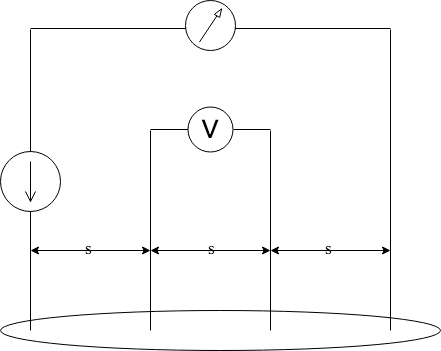
\includegraphics[scale=0.3]{FourPoint.png}
  \caption[Autocorrelations after PCA]{Dimensionally-reduced spatial correlations}
  \label{fig:pca}
\end{figure}

\subsection{Partial least squares analysis}

Unfortunately, due to the homogeneity of the samples as shown by the two point spatial correlations, no partial least squares model can be made from the data to capture the difference in sheet resistance.
